\chapter{Lineamientos para el desarrollo del sistema operativo}

El CDP1802 ya cuenta con algunos sistemas operativos funcionales, los mismos pueden probarse en el simulador Emma02. Entre ellos está el ElfOS\cite{elfOSr}, el cual utilizamos como guía para describir algunas características a esperarse de tal sistema.

El sistema operativo a desarrollarse debe contar con un sistema de archivos, el cual incluya directorios y la posibilidad de navegar en ellos. Como ejemplo, el ElfOS, posee los comandos DIR y CHDIR, los cuales tienen la función de visualizar y cambiar el directorio, respectivamente. En la figura~\ref{F:dir_chdir} puede verse como ejemplo la ejecución de estos dos comandos.

\begin{figure}[H]
  \centering
  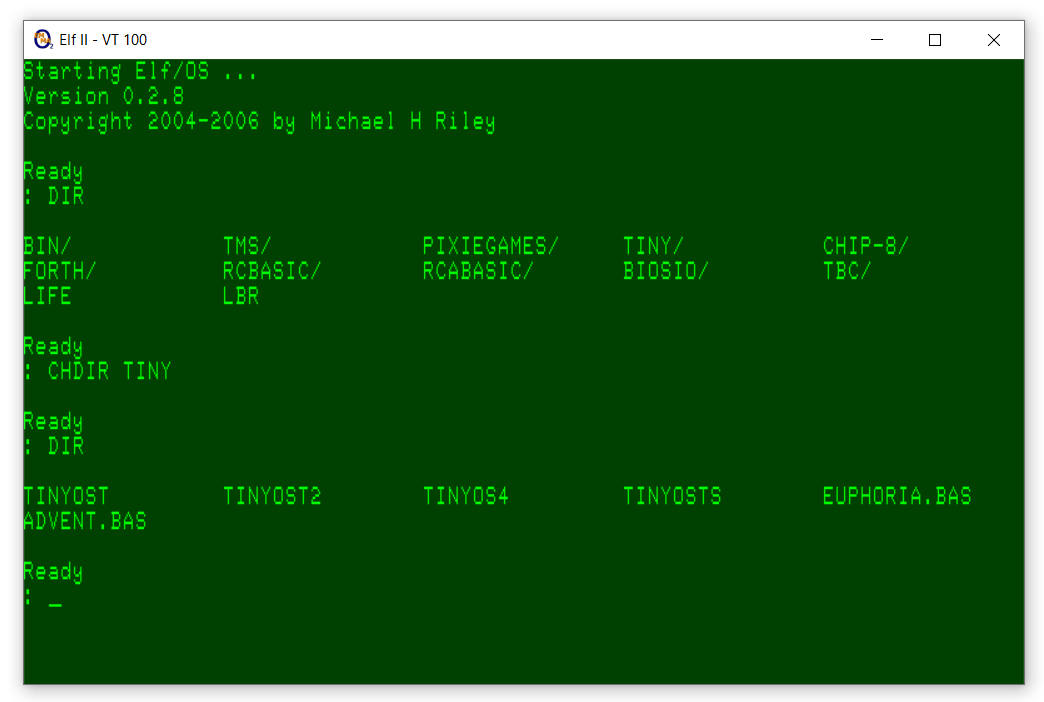
\includegraphics[width=0.95\textwidth]{./imagenes/dir_chdir.png}
  \caption{Sistema de directorios del ElfOS}
  \label{F:dir_chdir}
\end{figure}

El sistema operativo también debe incluir programas para crear y editar archivos de texto. El ElfOS posee este programa, que además brinda la posibilidad de escribir código en el lenguaje ensamblador del CDP1802, el cual puede luego ser ejecutado dentro del mismo sistema operativo, retomando su operación una vez ejecutado el código.

El sistema debe funcionar mediante el envío y recepción de caracteres (sin interfaz gráfica) mediante la comunicación con una terminal externa. Existen módulos conversores de protocolo Serial a USB que permiten realizar esta tarea.

El sistema no debe incluir conexión a internet ni ser multiusuario.

Debe contemplarse la posibilidad de que el sistema operativo a desarrollar sea de tiempo real (\textit{Real-Time Operating System RTOS}). Esto significa que debe ser capaz de aceptar y responder a eventos externos con cierto grado de fiabilidad, y en un margen de tiempo específico. Esta cualidad permite utilizar el sistema en aplicaciones industriales, donde se requiere atender a gran número de eventos externos y además controlar variables externas. La implementación de un sistema operativo de estas características permitiría utilizar la microcomputadora como un PLC.